\documentclass[12pt]{article}
\usepackage{graphicx}
\usepackage[latin1]{inputenc}
\usepackage{amsmath}
\usepackage{calc}
\usepackage{amssymb}

\textwidth = 15.5 true cm
\topmargin=-1.0truecm
\evensidemargin=0pt
\oddsidemargin=0pt
\parindent=0pt
\frenchspacing
\pagestyle{empty}

\newcommand{\HRule}{\rule{\linewidth}{0.075mm}}

\newlength{\depthofsumsign}
\setlength{\depthofsumsign}{\depthof{$\sum$}}
\newcommand{\nsum}[1][1.4]{\mathop{\raisebox{-#1\depthofsumsign+1\depthofsumsign}{\scalebox{#1}{$\displaystyle\sum$}}}}

\begin{document}

\parbox[t]{8cm}{\textsf{Course 02249 Computationally Hard Problems\\
Fall 2013, DTU Compute }}
\hfill
\parbox[t]{1cm}{\mbox{}\\
\raisebox{0.0cm}[1cm][1cm]{
\includegraphics[origin=lb]{dtu_logo.pdf}}}

{\Large  Solution to assignment \textsc{Project}\\[4mm]
Students' names: Andreas Hallberg Kjeldsen and Morten Chabert Eskesen\\[4mm]
Study nr. s092638 and s133304\\[4mm]
Date. 04\textbf{.}11\textbf{.}2013 }


\vspace{7cm}

\begin{center}
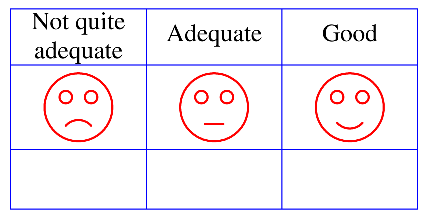
\includegraphics[scale=1.0]{Evurd.pdf}
\end{center}

\newpage

\HRule\\
\textbf{Problem:} \textsc{[MirrorFriendlyMinimumSpanningTree (MFMST)]}\\
\textbf{Input:} An undirected, connected weighted graph $G = (V,E,w)$, where $V = \{1,\dots,n\}$, $E = \{e_1,\dots,e_m\}$ and $w : E \rightarrow \mathbb{N}_0$, and a number $B \in \mathbb{N}$.\\
\textbf{Output:} YES if there is a spanning tree $T \subseteq E$ for $G$ such that
$$max \left\{\nsum\limits_{e_i \in T} w(e_i), \nsum\limits_{e_i \in T} w(e_{m+1-i})\right\} \leq B$$
and NO otherwise.\\
\HRule

\subsection*{a) Description of the problem in colloquial terms}
A minimum spanning tree is a subgraph within a undirected, connected weighted graph that is a tree and connects all the vertices together with a weight less or equal to the weight of every other spanning tree. The main difference between a minimum spanning tree and a mirror friendly minimum spanning tree is the inequality described above. In a mirror friendly minimum spanning tree the inequality must be satisfied. It should be possible to mirror the spanning tree in such a way that the maximum of the spanning tree and the mirrored spanning tree is less than or equal to a fixed value, $B$. This also means that the mirror friendly minimum spanning tree may not be equal to the minimum spanning tree in the graph, i.e. it may have a larger weight than the minimum spanning tree.

\subsubsection*{Solve an example problem}
\textbf{Input:} $V = \{1,2,3\}$, $E = \{e_1 = \{1,2\},e_2 = \{2,3\},e_3 = \{1,3\}\}$, $w(e_i) = i$ for $i \in \{1,2,3\}$ and $B = 4$.
\begin{center}
\begin{tabular}{ c c }
Spanning Tree & Mirrored Spanning Tree\\
$e_1 + e_2 = 3$ & $e_{3+1-1} + e_{3+1-2} = 5$\\
$e_3 + e_1 = 4$ & $e_{3+1-3} + e_{3+1-1} = 4$\\
\end{tabular}
\end{center}
$$max \left\{e_3 + e_1, e_{3+1-3} + e_{3+1-1}\right\} \leq 4$$
$$max \left\{4, 4\right\} \leq 4$$
Output would be a spanning tree consisting of the edges: $e_3$ and $e_1$.
\subsection*{b) Show that MFMST is in $NP$}
\subsubsection*{1. Design a deterministic algorithm $A$ which takes as input a problem instance $X$ and random sequence $R$}
\textbf{Specify what the random sequence $R$ consists of}\\
Let the string $R$ consist of bits: $R = r_1,r_2,\dots,r_n$.\\[0.25cm]
\textbf{Specify how $A$ interprets $R$ as a guess}\\
Consider the first $m$ bits. If the $i$-th bit is 1, mark the edge $e_i$.\\[0.25cm]
\textbf{Specify how $A$ verifies the guess}\\
If the marked edges create a mirror friendly minimum spanning tree with a weight less than or equal to $B$, answer YES, otherwise NO.
\subsubsection*{2. Show that the two conditions are met}
\textbf{If the answer to $X$ is YES, then there is a string $R^*$ with positive probability such that $A(X, R^*) = YES$}
\begin{itemize}
\item[] Asssume that the answer is YES
\item[] Then there is a subset of the edges that creates a mirror friendly minimum spanning tree with a weight less than or equal to $B$.
\item[] Let $S \subseteq \{1,\dots,m\}$ be the set that describe the edges' index
\item[] Construct the bit string $R^* = r_1,r_2,\dots,r_m$ where $r_i = 1$ if and if only if $i \in S$
\item[] When $A$ receives $R^*$, it will select the edges in $S$, check that the weight of the edges are less than or equal to $B$ and answer YES.
\item[] Altogether there is a string of length at most $p(n)$ that will give YES. The probability of randomly creating it is positive.
\end{itemize}
\textbf{If the answer to $X$ is NO, then $A(X, R) = NO$ for all $R$}
\begin{itemize}
\item[] Assume that the answer is NO
\item[] Then no set of the edges create a mirror friendly minimum spanning tree with a weight less than or equal to $B$.
\item[] If $R$ does not contain enough bits, the algorithm will correctly answer NO.
\item[] Otherwise the algorithm will mark some edges and compute their weight. This will be compared to $B$. But as no set of edges has a weight less than or equal to $B$, the answer is NO.
\end{itemize}
\subsubsection*{3. Show that $A$ is $p$-bounded for some polynomial $p$}
\begin{itemize}
\item[] There are $m$ edges.
\item[] It is checked that the string $R$ consists of at least $m$ bits. Time: $O(m)$.
\item[] Every edge is marked or not marked. Time: $O(m)$.
\item[] The weights of the marked edges are added. Time: $O(m)$.
\item[] The computed total weight is compared to $B$ and the answer is returned. Time: $O(1)$.
\end{itemize}
Altogether the time is: $O(m)$.
\subsection*{c) Show that MFMST is $NP$-complete}
\subsubsection*{Suitable problem $P_c$ known to be $NP$-complete}
\HRule\\
\textbf{Problem:} \textsc{[1-In-3-Satisfiability]}\\
\textbf{Input:} A set of clauses $C = \{c_1,\dots,c_k\}$ over $n$ boolean variables $x_1,\dots,x_n$, where every clause contains exactly three literals.\\
\textbf{Output:} YES if there is a satisfying assignment such that every clause has exactly one true literal, i.e., if there is an assignment
$$a: \{x_1,\dots,x_n\} \rightarrow \{0,1\}$$
such that every clause $c_j$ is satisfied and no clause has two or three satisfied literals, and NO otherwise.\\
\HRule\\
Prove $\textsc{1-In-3-Satisfiability} \leq_p$ \textsc{MirrorFriendlyMinimumSpanningTree}.\\
In order to prove this we use component design. When given an instance $(X,C)$ of \textsc{1-In-3-Satisfiability} we construct an instance $(G = (V, E,w),B)$ of MFMST. This is done by building small "component" graphs that are later connected to form the desired graph $G$. The components will have different "responsibilities". Some ensure a correct setting of the truth values, others which test satisfiability and components to connect them.
\\[0.25cm]\textbf{Outline of the transformation}\\
Let $X = \{x_1,\dots,x_n\}$ be the boolean variables and $C = \{c_1,\dots,c_m\}$ the clauses over $X$. We set $B = n + 2m$ for the MFMST instance. We set $w(e_i) = i$. The vertex set of $G$:
$$V = \{x_1,\dots,x_n\} \cup \{\overline{x}_1,\dots,\overline{x}_n\} \cup \bigcup_{j=1}^{m}{\{a_1(j),a_2(j),a_3(j)\}}$$
The truth setting components are defined to be the edges.
\begin{center}
$\forall x_1 \in X$ let $T_1$ be the vertex with incoming edges $x_1$ and $\overline{x}_1$
\end{center}
These components ensure that every spanning tree has to contain at least one of the edges $x_1$ or $\overline{x}_1$.\\
The components for clause satisfiability are defined by the following.
\begin{center}
$\forall c_j \in C$: let $S_j$ be the set of vertices\\
$S_j  = \{v_1(j),v_2(j),v_3(j)\}$
\end{center}
Two edges per triangle are needed to make a spanning tree. The edge not chosen is the \emph{true} literal which satisfies $c_j$.\\
The connecting components are defined by the following. Let $c_j = l_1 \vee l_2 \vee l_3$ where $l_k$ are literals. More specifically $l_k$ is a boolean variable $x_i$ or negated boolean variable $\overline{x}_i$. For every clause $c_j$ the following three vertices are added.
\begin{center}
$K_j = \{(v_1(j) \vee l_1), (v_2(j) \vee l_2), (v_3(j) \vee l_3)\}$
\end{center}
The vertex set $V$ is therefore:
$$V = \bigcup_{i=1}^{n}{T_i} \cup \bigcup_{j=1}^{m}{S_j} \cup \bigcup_{j=1}^{m}{K_j}$$
The transformation $T$ can be performed in time polynomial in $n$ and $m$.
\\[0.25cm] \textbf{Answer to $X$ is YES then answer to $T(X)$ is YES}\\
Assume that $a: X \rightarrow \{0,1\}$ is an assignment which satisfies all clauses $c_j$. Consider the graph $G = (V,E,w)$ constructed above. We begin to construct $T \subseteq E$ by selecting $n$ edges as follows:
\begin{center}
$x_i \in T \Longleftrightarrow a(x_i) = 1$,\\
$\overline{x}_i \in T \Longleftrightarrow a(x_i) = 0$.
\end{center}
Then all $T_i$ are covered. For every clause $c_j$ at least one connecting vertex is covered by an $l_k$ (by virtue of some literal in $c_j$ is set to 1). Assume that for clause $c_j$ this is $l_1$. We add $a_2(j)$ and $a_3(j)$ to $T$. These two edges cover the other two connecting vertices and the three vertices of the triangle $S_j$. The set $T$ is a spanning tree and has weight $B = n + 2m$.
\\[0.25cm] \textbf{Answer to $T(X)$ is YES then answer to $X$ is YES}\\
Lets assume that $T \subseteq E$ is a spanning tree for $G$ with a mirrored spanning tree where both have a weight less than or equal to $B$. In order to cover the vertices at least one of the edges $x_i$ or $\overline{x}_i$ has to be in $T$. In order to cover the vertices of $S_j$, the spanning tree $T$ has to contain at least two of the edges. Therefore $|T| = B = n + 2m$, and we have that $T$ contains exactly one edge from every $T_i$ and exactly two edge from every $S_j$.\\
We define an assignment: $a(x_i) =$ 1 if $x_i \in T$ and 0 if $\overline{x}_i \in T$\\
As $T$ contains exactly one of $x_i$ or $\overline{x}_i$ the assignment $a$ is well defined. We still need to show that the assignment satisfies all clauses $c_j$. Let $c_j = l_1 \vee l_2 \vee l_3$ be a clause where $l_k$ are literals. For every component $S_j$ exactly two edges belong to $T$, say $\{v_1(j),v_2(j)\}$ and $\{v_2(j),v_3(j)\}$. They cover also the connecting vertices $(v_1(j) \vee l_1)$ and $(v_2(j) \vee l_2)$. The third connecting vertex $(v_3(j) \vee l_3)$ attached to $S_j$ has to be covered by $l_3$. By the construction of $G$ $l_3$ corresponds to a literal in $c_j$ and by the construction of the assignment $a$, $l_3$ is set to true and clause $c_j$ is then satisfied because only one literal in a clause must be true.
\subsection*{d) Find an algorithm which solves the optimizing version of the problem}


\subsection*{e) Prove the worst-case running time of the algorithm}


\subsection*{f) Implement the algorithm developed in d)}


\end{document}
